\documentclass[10pt]{article}

% Manuscript v7 (draft, 21 Nov 2026). Restructured around what the evidence supports: the method, the
% LoCoMo comparison with a same-reader RAG baseline, the repair/abstention analysis with its break-even
% condition, and the first-stage-retriever finding. Results that did not support a claim (graph repair,
% hybrid repair, LongMemEval oracle) are not part of the headline and are reported in Appendix B and
% summarised in Section 6. The confirmatory LongMemEval-S run (protocol v3) was launched on 21 Nov 2026;
% its result is not in this draft.
\usepackage[letterpaper,margin=1in]{geometry}
\usepackage{times}
\usepackage{amsmath,amssymb,amsthm}
\usepackage{booktabs}
\usepackage{graphicx}
\usepackage{array}
\usepackage{multirow}
\usepackage{xcolor}
\usepackage{float}
\usepackage[round]{natbib}
\usepackage{hyperref}
\hypersetup{colorlinks=true,linkcolor=blue,citecolor=blue,urlcolor=blue}
\emergencystretch=2em

\theoremstyle{plain}
\newtheorem{proposition}{Proposition}
\newtheorem{lemma}{Lemma}
\newtheorem{theorem}{Theorem}
\newtheorem{corollary}{Corollary}

\newcommand{\care}{\textsc{CARE}}
\newcommand{\pending}[1]{\textcolor{red}{\textbf{[PENDING: #1]}}}
\newcommand{\A}{\mathcal{A}}

\title{\textbf{\care{}: Conditional Answer Repair with Source-Anchored Evidence\\
for Long-Horizon Conversational Question Answering}}
\author{Anonymous authors\\ \small Draft v7 --- not under review}
\date{}

\begin{document}
\maketitle

\begin{abstract}
A conversational agent must answer questions about histories far longer than its context window. We present
\care{}, a bounded reader over an append-only archive of the original turns. The reader answers with cited
turn identifiers; code verifies that every citation lies in the evidence it was shown and that first-person
claims are bound to the right speaker; and a gate driven by the reader's own structured output (an abstention,
or the searches it proposes) triggers at most one repair read on an expanded bundle. With open models only
(Qwen3-8B reader, Qwen3-Embedding-0.6B encoder), \care{} scores 0.526 on all 1,986 LoCoMo questions against 0.457
for a same-reader dense RAG baseline ($+0.069$, 95\% interval $[+0.042,+0.099]$, ahead in all ten
conversations) at 1.6 times the tokens, with the gain coming from single-hop ($+0.145$) and temporal ($+0.070$)
questions. Repair improves 279 questions and costs 46 correct refusals. We prove a break-even condition that any
acceptance verifier must meet to recover those refusals (it must catch refusal-losing repairs 3.89 times as often as it
rejects useful ones), and six verifiers we built fall short of it. A dense first-stage retriever helps before repair
but not after it. LoCoMo served for development, we do not compare with published memory systems, and a confirmatory
LongMemEval-S run is pending.
\end{abstract}

% =====================================================================================
\section{Introduction}
\label{sec:intro}

Agents that converse over months must answer questions whose evidence was said long ago, may have
been updated, or belongs to a particular speaker. Memory systems address this by writing structured notes
during the conversation \citep{packer2023memgpt,chhikara2025mem0,amem2025,memoryr12025,cao2026higmem}, or by
keeping the history and selecting evidence per question \citep{du2026memr3,wang2026cuemem,liu2026livectx,chen2026justmem,yu2026lazymem}.
Rewriting what was said loses the original wording, and nothing then lets the system check that an answer is
actually supported. Corrective retrieval reads again when a first answer looks unsupported
\citep{jiang2023active,asai2023selfrag,yan2024crag}, deciding from token confidence, a learned critique or a retrieval
evaluator. \care{} instead uses deterministic code checks on the answer's citations.

\care{} keeps the original turns as the only citable evidence and puts the verification in code. The reader must
cite turns; citations that are not in the bundle it was shown, or that attribute one speaker's first-person fact to
another, invalidate the answer; and an abstention that comes with concrete searches, or an invalidated answer,
triggers one more read on an expanded bundle. Our questions are narrow: how much does such a second read help, what
does it cost, and where does the benefit come from?

\paragraph{Contributions.}
\begin{enumerate}
  \item \textbf{A source-anchored bounded reader} (Section~\ref{sec:method}). An append-only archive of turns;
  citation and speaker-binding checks executed in code against the visible bundle; and a repair gate driven by the
  reader's own structured output rather than by a confidence score. At most two reader calls per question.
  \item \textbf{A same-reader comparison on LoCoMo} (Section~\ref{sec:results}). \care{} beats a dense RAG baseline
  with the same reader by $+0.069$ (all ten conversations; answerable questions $+0.089$), and the decomposition by
  question type shows where: single-hop and temporal questions.
  \item \textbf{A decomposition of repair into gain and abstention cost, with a break-even condition}
  (Section~\ref{sec:abstention}). Repair improves 279 questions and loses 46 correct refusals. We derive the rate at
  which an acceptance verifier must separate the two kinds of repair and show that six verifiers do not reach it.
  \item \textbf{Repair compensates for the first-stage retriever} (Section~\ref{sec:retriever}). A dense encoder
  beats BM25 before repair ($+0.014$) but not after it.
  \item \textbf{A pre-registered, open-model protocol} with exact reproduction of saved answers.
\end{enumerate}

\paragraph{Scope.} LoCoMo is our development set, so its numbers are not held-out. We did not reproduce published
memory systems under our reader and metric and make no claim about them. The memory write path is implemented and
unit-tested but not evaluated. Section~\ref{sec:discussion} lists what did not work.

% =====================================================================================
\section{Related Work}
\label{sec:related}

\paragraph{Persistent memory.} MemGPT pages information between context and storage \citep{packer2023memgpt}.
Mem0 extracts and consolidates facts \citep{chhikara2025mem0}; A-Mem links and revises notes \citep{amem2025};
Memory-R1 learns write operations \citep{memoryr12025}; HiGMem maintains an event--turn hierarchy and refreshes
summaries as turns arrive \citep{cao2026higmem}. These systems change what is stored; \care{} keeps the stored
text fixed and changes only how it is read.

\paragraph{Read-time access.} MemR$^3$ routes among retrieval and answering while tracking evidence gaps
\citep{du2026memr3}; CueMem and LiveCtx rebuild context from raw turns \citep{wang2026cuemem,liu2026livectx};
JustMem selects lookup, composition or replay per query \citep{chen2026justmem}; LazyMem builds compact memory
at query time \citep{yu2026lazymem}.

\paragraph{Corrective retrieval.} FLARE, Self-RAG, Adaptive-RAG and CRAG decide when to retrieve again
\citep{jiang2023active,asai2023selfrag,jeong2024adaptive,yan2024crag}. \care{} differs in two ways: its gate reads
the reader's structured self-report (an abstention plus proposed searches) and failures of deterministic citation checks
rather than a learned or model-based critique, and every final answer must cite turns that code has verified to be in the
evidence shown. We compare with none of these systems under a shared implementation.

% =====================================================================================
\section{Method: \care{}}
\label{sec:method}

\begin{figure}[t]
\centering
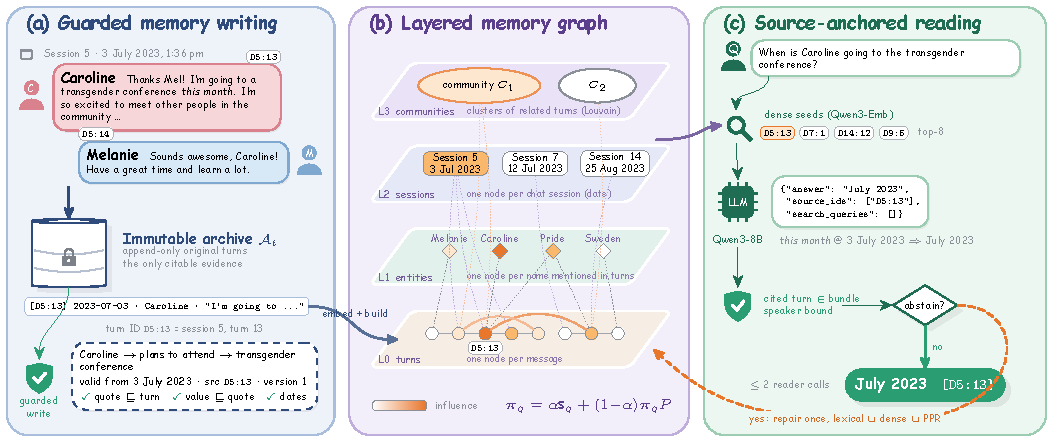
\includegraphics[width=\linewidth]{figures/asem_method_figure.pdf}
\caption{Overview. \textbf{(a)} Original turns enter an append-only archive, the only citable evidence; the write path
(guarded operators) is implemented but not part of any reported result. \textbf{(b)} An exploratory layered graph over
the archive; it is not part of the \care{} results and is described in Appendix~\ref{app:more}. \textbf{(c)} The reader
answers from a top-8 first bundle with cited identifiers, code checks bind the citations to the bundle, and an
abstention with searches triggers at most one repair. The example is a saved output of our run (LoCoMo
\texttt{conv-26}, question 17).}
\label{fig:overview}
\end{figure}

\subsection{Archive and first bundle}

A conversation is a stream of turns $s_i=(\mathrm{id}_i,\sigma_i,t_i,p_i,x_i)$ with session $\sigma_i$, date
$t_i$, speaker $p_i$ and text $x_i$. The archive $\A_t=\{s_i:i\le t\}$ is append-only and is the only source a
final answer may cite. The first bundle $B_1$ is the top eight turns under BM25 (a dense ranking is an option,
Section~\ref{sec:retriever}), serialized with identifier, date and speaker under $L=10{,}000$ characters. BM25 uses
$k_1{=}1.5$ and $b{=}0.75$.

\subsection{Reader, source checks and gate}

The frozen reader returns an answer $a_1$, cited identifiers $C_1$ and at most two searches $Q_1$:
\begin{equation}
(a,\,C,\,Q)=R_\theta(q,B),\qquad C\leftarrow C\cap\mathrm{ids}(B),\qquad a\leftarrow\bot\ \text{if } C=\varnothing.
\label{eq:reader}
\end{equation}
Three code checks can invalidate an answer that cites turns ($r=1$): a speaker-binding check for questions naming one
speaker, and two event checks (holiday names, cessation verbs). Repair fires when
\begin{equation}
\tau(q)=\mathbf{1}\big[r_1\ \lor\ \big(a_1=\bot\ \land\ (Q_1\neq\varnothing\ \lor\ \rho(q))\big)\big],
\label{eq:gate}
\end{equation}
where $\rho$ flags temporal, update or aggregation cues. Each question uses $1+\tau(q)\le 2$ reader calls. In our traces
the reader's own output drives the gate: of the 1,004 repairs on LoCoMo, 867 followed an abstention with proposed
searches and 137 followed an invalidated answer; $\rho$ was never the only trigger.

\subsection{Repair read}

When $\tau(q)=1$ the reader is called once more on an expanded bundle $E(q,Q_1)$: the top 18 unstemmed and stemmed
BM25 turns for the question, the session neighbours of the leading hits, and six unstemmed and six stemmed hits for
each proposed search. The expanded pool is restored to conversation order and cut at $L$ characters. The prompt adds
a correction that depends on why the first read failed (a speaker-binding failure, or missing direct evidence). The
second answer is checked in the same way and is final.

\subsection{Write path (implemented, not evaluated)}

Versioned notes can be added or updated only through operators whose guards are checked in code: a quote must be an
exact substring of a cited turn, the value must occur in the quote, and updates are ordered by parsed dates. Rejected
writes are logged. These operators have 15 unit tests but are not part of any reported result.

% =====================================================================================
\section{Experimental Setup}
\label{sec:setup}

\paragraph{Data.} \emph{LoCoMo} \citep{maharana2024locomo}: ten conversations, 5,882 turns, 1,986 questions in five
categories (multi-hop 282, temporal 321, open-domain 96, single-hop 841, adversarial 446). LoCoMo was used to develop
\care{}, so it is a development set. \emph{LongMemEval} \citep{wu2024longmemeval} was used for a secondary check
(Section~\ref{sec:discussion}, Appendix~\ref{app:more}). A confirmatory run on LongMemEval-S (full histories) is
specified in protocol v3 and was launched on 21 November 2026; \pending{result not in this draft}.

\paragraph{Systems.} All systems share the reader, decoding, evidence cap and citation checks.
\textbf{NoMemory}: no history. \textbf{FullContext-8K}: the first five turns and the most recent suffix that fit in an
8K window (truncated, not a full-context system). \textbf{RAG}: dense top-18 turns in a plain prompt, one call.
\textbf{\care{} first pass}: BM25 top-8 bundle, no repair. \textbf{\care{}}: first pass plus the conditional repair
above.

\paragraph{Metrics.} The LoCoMo benchmark scorer: per-item F1 for multi-hop questions, stemmed-token F1 for the other
answerable categories, and a refusal phrase match for adversarial questions; the aggregate is the mean per-question
score. We also report the answerable-question score, correct refusals (of 446 unsupported questions), answerable
questions answered with $\bot$, calls, and server-counted input plus output tokens. Intervals are paired bootstraps that
resample conversations (10,000 draws); with ten conversations they are optimistic, so we also report how many
conversations favour each contrast.

\paragraph{Implementation and reproducibility.} Qwen3-8B reader (pinned revision, fp16, vLLM, non-thinking, temperature
0, at most 224 output tokens, 8,192-token window) on two T4 GPUs; Qwen3-Embedding-0.6B encoder (pinned, fp16, documents
at most 1,024 tokens). All models are open weights. The factorial worker reproduces the saved \care{} answers exactly on
all 1,986 LoCoMo questions, and the GPU dense top-8 matches the frozen rankings on 99.7\% of entries. Gold labels enter
only after inference. The study followed a registered protocol (Appendix~\ref{app:protocol}).

% =====================================================================================
\section{Results}
\label{sec:results}

\subsection{\care{} against baselines on LoCoMo}

\begin{table}[t]
\centering
\caption{All systems on the same 1,986 LoCoMo questions. ``Refused ans.'' counts answerable questions answered with
$\bot$ (of 1,540). Tokens are server-counted input plus output per question.}
\label{tab:main}
\small
\begin{tabular}{lrrrrrr}
\toprule
System & Score & Answerable & Correct refusals & Refused ans. & Calls & Tokens/q \\
\midrule
NoMemory & 0.077 & 0.100 & 0/446 & 2 & 1,986 & 78 \\
FullContext-8K (truncated) & 0.196 & 0.241 & 19/446 & 40 & 1,986 & 7,888 \\
RAG dense top-18 & 0.457 & 0.376 & 327/446 & 271 & 1,986 & 1,180 \\
\midrule
\care{} first pass (BM25) & 0.459 & 0.349 & 374/446 & 630 & 1,986 & 715 \\
\care{} & \textbf{0.526} & \textbf{0.465} & 328/446 & 257 & 2,990 & 1,836 \\
\bottomrule
\end{tabular}
\end{table}

\care{} improves on every baseline (Table~\ref{tab:main}). Against the same-reader RAG baseline the difference is
$+0.069$ (interval $[+0.042,+0.099]$, ahead in 10 of 10 conversations); on the 1,540 answerable questions it is
$+0.089$ ($[+0.070,+0.108]$). Repair accounts for the gain over the first pass ($+0.067$, $[+0.050,+0.085]$, 10 of 10
conversations; 279 questions improve and 46 decline), and it costs 1.6 times the tokens of RAG (1,836 against 1,180
per question) and 1.5 calls per question. The truncated 8K full-context baseline is not a fair test of reading the
whole history: a 30K-token baseline is \pending{not yet run}.

\begin{table}[t]
\centering
\caption{Score by LoCoMo question type. Last columns: \care{} minus RAG with the conversation-cluster 95\% interval.}
\label{tab:category}
\small
\begin{tabular}{lrrrrr}
\toprule
Type (n) & RAG & \care{} first pass & \care{} & \care{} $-$ RAG & 95\% interval \\
\midrule
Single-hop (841) & 0.431 & 0.432 & \textbf{0.576} & $+0.145$ & $[+0.116,+0.174]$ \\
Temporal (321) & 0.371 & 0.372 & \textbf{0.441} & $+0.070$ & $[+0.018,+0.135]$ \\
Open-domain (96) & 0.159 & 0.100 & 0.165 & $+0.006$ & $[-0.081,+0.076]$ \\
Adversarial (446) & 0.733 & 0.839 & 0.735 & $+0.002$ & $[-0.067,+0.072]$ \\
Multi-hop (282) & 0.293 & 0.159 & 0.261 & $-0.032$ & $[-0.079,+0.010]$ \\
\bottomrule
\end{tabular}
\end{table}

Table~\ref{tab:category} shows where the gain comes from. The two largest categories that need one specific piece of
evidence, single-hop and temporal questions, improve by $+0.145$ and $+0.070$, and the intervals exclude zero. On
open-domain and adversarial questions \care{} ties with RAG, and on multi-hop questions it is below RAG, although the
interval contains zero. Adversarial questions show the trade-off studied next: the first pass scores 0.839 because it
refuses, and repair lowers this to 0.735.

\subsection{Repair buys answers with refusals: a break-even condition}
\label{sec:abstention}

Repair raises the score by $+0.067$: 279 questions improve and 46 correct refusals are lost, where the first pass
refused correctly and the repair produced an unsupported answer. Of the 1,004 repairs, 419 changed the outcome (373 on
answerable questions, 46 on unsupported ones). A verifier that keeps a subset of those 419 flips changes the total score
relative to accepting all of them by $L^{\mathrm{caught}}_V-G^{\mathrm{rej}}_V$ (Theorem~\ref{thm:breakeven}): the
refusals it saves minus the gains it throws away. With total gain $G=179.11$ and $L=46$ losses, a verifier that rejects
flips independently of their value improves on accepting everything only if its rejection rate on unsupported flips
exceeds its rejection rate on answerable flips by a factor of $G/L=3.89$ (Corollary~\ref{cor:rate}).

\begin{table}[t]
\centering
\caption{Verifiers on the 419 LoCoMo flips (Qwen3-8B). $\alpha$ is the share of unsupported flips rejected, $\beta$ the
share of answerable flips rejected. Every verifier lowers the score relative to accepting all flips. ``Think'' denotes
Qwen3 thinking mode; R1--R4 are the acceptance rules in Appendix~\ref{app:verifiers}.}
\label{tab:verify}
\small
\begin{tabular}{lrrrr}
\toprule
Verifier & $\alpha$ & $\beta$ & $\alpha/\beta$ & $\Delta_V-\Delta_{\mathrm{all}}$ \\
\midrule
Accept all & 0 & 0 & -- & 0 \\
Oracle (uses gold; ceiling) & 1 & 0 & $\infty$ & $+46.00$ \\
\midrule
Yes/no & 0.196 & 0.129 & 1.52 & $-8.05$ \\
Quote-grounded, no think, R3 & 0.261 & 0.279 & 0.94 & $-26.95$ \\
Quote-grounded, no think, R4 & 0.065 & 0.043 & 1.52 & $-3.04$ \\
Quote-grounded, think, R1 & 0.761 & 0.445 & 1.71 & $-32.62$ \\
Quote-grounded, think, R3 (pre-registered) & 0.761 & 0.496 & 1.53 & $-42.52$ \\
Quote-grounded, think, R4 & 0.717 & 0.311 & 2.31 & $-16.80$ \\
\bottomrule
\end{tabular}
\end{table}

Six verifiers fall below the 3.89 bound and all lower the score (Table~\ref{tab:verify}). Thinking-mode verifiers do
recognise unsupported premises when asked to quote them (35 of 46 refusal-losing flips caught) but they also reject 185
of 373 useful flips. The measured losses are always smaller than the independence prediction, so the verifiers do prefer
to reject low-value flips, but not enough. Fourteen label-free trace features separate the two kinds of flip with AUC at
most 0.60. The practical consequence is that the abstention cost is structural: recovering it needs a verifier that
separates the two kinds of flip about 1.7 times better than the best we built (3.89 against 2.31).

\subsection{Repair compensates for the first-stage retriever}
\label{sec:retriever}

\begin{table}[t]
\centering
\caption{Recall of annotated evidence in the top-$k$ ranking on LoCoMo, without a reader.}
\label{tab:retrieval}
\small
\begin{tabular}{lcc}
\toprule
Ranker & $k{=}8$ & $k{=}18$ \\
\midrule
BM25 & 0.539 & 0.624 \\
Dense (Qwen3-Embedding-0.6B) & \textbf{0.617} & \textbf{0.725} \\
Hybrid RRF & 0.612 & -- \\
\bottomrule
\end{tabular}
\end{table}

With Qwen3-Embedding-0.6B the dense ranking beats BM25 at both depths (Table~\ref{tab:retrieval}), in all ten
conversations; an earlier comparison with MiniLM-L6-v2 had favoured BM25, so that conclusion does not survive a
stronger encoder. A dense first bundle also raises the score before repair, from 0.459 to 0.473 ($+0.014$, interval
$[+0.007,+0.023]$, 9 of 10 conversations). After repair the advantage does not carry over: a dense first bundle with
the same repair scores 0.518 against 0.526 for BM25 ($-0.008$, $[-0.017,+0.001]$). Repair therefore removes most of the
sensitivity of the final score to the first-stage ranker, which makes \care{} cheap to deploy with a lexical index only.

% =====================================================================================
\section{Discussion and Limitations}
\label{sec:discussion}

\paragraph{What the evidence supports.} On LoCoMo, reading original turns with checked citations and one bounded repair
beats a same-reader dense RAG baseline by about 0.07, with a decomposition that locates the gain in single-hop and
temporal questions. Repair buys answers with refusals, and the trade-off is structural: the total value of useful repairs
is about 3.9 times the number of harmful ones, so cheap verifiers cannot recover the lost refusals. The final score is
insensitive to whether the first bundle is lexical or dense.

\paragraph{What did not work or is not established.} We report these so that the claims above are read in context.
(i) A layered memory graph used for repair evidence, and a hybrid (lexical plus dense) repair expansion, gave no
measurable gain over lexical repair under the registered decision rule (Appendix~\ref{app:more}). The best development
score, 0.541 for hybrid repair, was selected after inspecting development results and is not confirmed. (ii) On the
LongMemEval cleaned-oracle set, where each history contains only the relevant sessions, a dense RAG baseline (0.424) and a
truncated full-context baseline (0.471) score above \care{} (0.383); the oracle setting favours reading over retrieval and
does not test memory retrieval, which is why the LongMemEval-S run was specified. (iii) \care{} is below RAG on multi-hop
questions (Table~\ref{tab:category}).

\paragraph{Limitations.} (a) LoCoMo was used for development, so its numbers are not held-out. (b) The LongMemEval metric
is a diagnostic token F1, not the official judged accuracy. (c) We use one reader, Qwen3-8B, with thinking disabled.
(d) The full-context baseline is truncated to 8K tokens. (e) We did not reproduce published memory systems, so no claim
about them is made. (f) The write path, the aggregation operator and memory evolution are not evaluated. (g) Intervals on
LoCoMo resample ten conversations and are therefore optimistic. (h) The repair gate contains LoCoMo-motivated code checks
(holiday and cessation cues); their contribution has not been ablated. \pending{mechanism ablation and LongMemEval-S
confirmatory run}

\section{Conclusion}

\care{} keeps original turns as the only citable evidence, verifies citations in code, and repairs once. On LoCoMo it
beats a same-reader dense RAG baseline by 0.069 in all ten conversations, mostly on single-hop and temporal questions, and
the analysis of its repair step gives a break-even condition showing why the abstention cost cannot be recovered by cheap
verification. The confirmatory test on full-history LongMemEval-S and an ablation of \care{}'s own components are the
next steps.

% =====================================================================================
\bibliographystyle{plainnat}
\bibliography{asem}

\appendix

\section{Properties and Proofs}
\label{app:proofs}

\begin{proposition}[Citable bundles]\label{prop:projection}
Under an append-only archive and exact guards, every bundle consists of archive turns, so every citation the
reader returns is an archive turn. Each question uses at most two reader calls.
\end{proposition}
\begin{proof}
Bundles are prefixes of rankings over $\A_t$; citations are filtered to the bundle by code; the second call
occurs only when $\tau(q)=1$, and no further call is defined.
\end{proof}

\begin{theorem}[Break-even]\label{thm:breakeven}
For a verifier $V$ on flips, $\Delta_V-\Delta_{\mathrm{all}}=L^{\mathrm{caught}}_V-G^{\mathrm{rej}}_V$, where
$L^{\mathrm{caught}}_V$ counts rejected unsupported flips and $G^{\mathrm{rej}}_V$ sums the score gains of rejected
answerable flips.
\end{theorem}
\begin{proof}
$\Delta_{\mathrm{all}}-\Delta_V=\sum_{V(f)=0}d_f=G^{\mathrm{rej}}_V-L^{\mathrm{caught}}_V$, since $d_f=-1$ on unsupported
flips and $d_f\ge0$ on answerable ones.
\end{proof}

\begin{corollary}[Rate condition]\label{cor:rate}
If $V$ rejects unsupported flips with probability $\alpha$ and answerable flips with probability $\beta$,
independently of $d_f$, then $\mathbb{E}[\Delta_V-\Delta_{\mathrm{all}}]=\alpha L-\beta G$, and $V$ helps in
expectation iff $\alpha/\beta>G/L$.
\end{corollary}
\begin{proof}
Apply linearity of expectation to Theorem~\ref{thm:breakeven}.
\end{proof}

\begin{proposition}[Grounding and version chains]\label{prop:grounding}
Under an append-only archive and exact guards, every stored value is a substring of an archive turn, and each
key has at most one current note whose versions have non-decreasing validity dates.
\end{proposition}
\begin{proof}
\textsc{Add} and \textsc{Update} insert a note only after checking that the quote occurs in an archive turn, that the
value occurs in the quote, and (for \textsc{Update}) that exactly one current note exists and the new date is not
earlier. Other operations do not change notes.
\end{proof}

\section{Additional Results (not part of the headline claims)}
\label{app:more}

\paragraph{Variants.} The registered study crossed the first bundle (BM25 or dense) with the repair expansion. Besides the
lexical expansion of Section~\ref{sec:method}, two variants add a second ranker, with $D_k$ the top-$k$ dense ranking and
$G_k$ the top-$k$ ranking of the graph score $r_q(i)=\lambda z(\mathrm{sim}(q,i))+(1-\lambda)z(\pi_q(i))$ ($\lambda=0.7$):
\begin{align}
E_{\mathrm{hyb}}&=E_{\mathrm{lex}}\ \cup\ D_6(q)\ \cup\ \textstyle\bigcup_{s\in Q_1}D_6(s),\\
E_{\mathrm{graph}}&=E_{\mathrm{lex}}\ \cup\ G_6(q)\ \cup\ \textstyle\bigcup_{s\in Q_1}G_6(s).
\end{align}
The graph has turn nodes (\textsf{next} edges within a session, 5-nearest-neighbour semantic edges), entity nodes
(capitalized tokens in 2 to 5\% of turns), session nodes and Louvain community nodes (fixed seed); $\pi_q$ is the
personalized PageRank (restart $\alpha=0.5$) from the five best dense turns, built without an LLM. The locality bound
$\sum_{v\notin H_h}\pi_q(v)\le(1-\alpha)^{h+1}$ holds (Lemma~\ref{lem:ppr}).

\begin{lemma}[Locality of PPR]\label{lem:ppr}
Let $H_h$ be the nodes within $h$ hops of the seeds. Then $\sum_{v\notin H_h}\pi_q(v)\le(1-\alpha)^{h+1}$.
\end{lemma}
\begin{proof}
$\boldsymbol\pi_q=\alpha\sum_{\ell\ge0}(1-\alpha)^{\ell}\mathbf{s}_qP^{\ell}$, and $\mathbf{s}_qP^{\ell}$ is supported
within $\ell$ hops, so the mass outside $H_h$ is at most $\alpha\sum_{\ell>h}(1-\alpha)^{\ell}=(1-\alpha)^{h+1}$
\citep{andersen2006local}. Personalized PageRank was applied to long-term memory by \citet{gutierrez2024hipporag}.
\end{proof}

\begin{table}[t]
\centering
\caption{Registered factorial on the 1,986 LoCoMo questions (development). CARE-H adds dense evidence to the repair;
Dense-CARE uses a dense first bundle; CARE-G replaces the dense ranker in the repair by the graph ranker.}
\label{tab:factorial}
\small
\begin{tabular}{lrrrrrr}
\toprule
System & Score & Answerable & Correct refusals & Refused ans. & Calls & Tokens/q \\
\midrule
\care{} (BM25, lexical repair) & 0.526 & 0.465 & 328/446 & 257 & 2,990 & 1,836 \\
CARE-H (BM25, hybrid repair) & \textbf{0.541} & \textbf{0.486} & 325/446 & 210 & 2,990 & 1,976 \\
Dense first pass & 0.473 & 0.377 & 358/446 & 470 & 1,986 & 751 \\
Dense-CARE (lexical repair) & 0.518 & 0.464 & 313/446 & 221 & 2,814 & 1,681 \\
Dense-CARE-H (hybrid repair) & 0.520 & 0.470 & 309/446 & 190 & 2,814 & 1,801 \\
CARE-G (graph repair) & 0.520 & 0.471 & 307/446 & 193 & 2,814 & 1,799 \\
\bottomrule
\end{tabular}
\end{table}

\begin{table}[t]
\centering
\caption{Pre-registered hypotheses. The Bonferroni column uses 98.75\% for four tests; ``supported'' requires it to
exclude zero. LongMemEval is the cleaned oracle set with a diagnostic metric.}
\label{tab:hyp}
\small
\begin{tabular}{lrrrl}
\toprule
Contrast & Mean & 95\% interval & Bonferroni interval & Verdict \\
\midrule
\multicolumn{5}{l}{\emph{LoCoMo (development)}} \\
H1: Dense-CARE-H $-$ CARE & $-0.005$ & $[-0.017,\ +0.008]$ & $[-0.019,\ +0.012]$ & not supported \\
H2: Dense-CARE-H $-$ Dense-CARE & $+0.003$ & $[-0.003,\ +0.009]$ & $[-0.004,\ +0.010]$ & not supported \\
H3: Dense first pass $-$ BM25 first pass & $+0.014$ & $[+0.007,\ +0.023]$ & $[+0.005,\ +0.026]$ & \textbf{supported} \\
H4: CARE-G $-$ Dense-CARE-H & $-0.001$ & $[-0.007,\ +0.006]$ & $[-0.008,\ +0.007]$ & not supported \\
\midrule
\multicolumn{5}{l}{\emph{LongMemEval cleaned oracle}} \\
H1: Dense-CARE-H $-$ CARE & $+0.018$ & $[-0.006,\ +0.043]$ & $[-0.012,\ +0.050]$ & not supported \\
H2: Dense-CARE-H $-$ Dense-CARE & $+0.005$ & $[0.000,\ +0.012]$ & $[0.000,\ +0.014]$ & not supported \\
H3: Dense first pass $-$ BM25 first pass & $+0.014$ & $[-0.014,\ +0.044]$ & $[-0.022,\ +0.052]$ & not supported \\
H4: CARE-G $-$ Dense-CARE-H & $0.000$ & -- & -- & not informative \\
\bottomrule
\end{tabular}
\end{table}

Table~\ref{tab:factorial} gives the scores and Table~\ref{tab:hyp} the registered tests. Only H3 on LoCoMo is supported. The best development variant, CARE-H, is a post-hoc finding: CARE-H minus \care{} is
$+0.015$ on LoCoMo ($[+0.007,+0.025]$) and $+0.005$ on LongMemEval ($[-0.001,+0.013]$, not significant). H4 is not
informative on LongMemEval: CARE-G changed the repair bundle in only 9 of 500 questions compared with Dense-CARE-H,
because the oracle histories are short (about 25 turns). On LongMemEval oracle, the dense RAG baseline scores 0.424 and
the truncated full-context baseline 0.471, above every memory variant (\care{} 0.383, CARE-H 0.389, Dense-CARE-H 0.401).
The graph ranking is no better than the dense ranking at eight turns (recall 0.618 against 0.617) and adds about 0.01
at eighteen (0.736 against 0.725); the value of $\lambda$ was chosen on these development numbers.

\section{Protocol History and Deviations}
\label{app:protocol}

The factorial protocol (\texttt{docs/CARE\_factorial\_protocol\_20261117.md}) registered arms, metrics and H1--H3
before its full run. Amendment 1 added the graph arm and H4, before any full-run result was seen. Amendment 2
lowered the encoder batch from 8,192 to 2,048 tokens after out-of-memory failures on long histories. Seven of the
ten shards ran with 8,192 and three (LongMemEval shards 3 and 4, LoCoMo shard 4) with 2,048; in both groups the \care{}
arm reproduces the saved answers exactly. The LongMemEval oracle results were observed before the choice of CARE-H was
discussed. Protocol v3 (\texttt{docs/CARE\_protocol\_v3\_20261118.md}) fixes the confirmatory LongMemEval-S test, whose
only primary hypothesis is CARE-H $-$ \care{} $>0$, before any shard ran; it was launched on 21 November 2026.

\section{Verifier Details}
\label{app:verifiers}

R1 accepts a flip iff the verifier's verdict is \textsc{supported}; R2 also requires a valid answer quote; R3
requires valid answer and premise quotes; R4 rejects only \textsc{premise-unsupported}. In thinking mode, three
replies reached the token limit and two could not be parsed; these count as rejections under R1 to R3 and as
acceptances under R4.

\section{Provenance of Reported Numbers}
\label{app:provenance}

{\footnotesize
\begin{tabular}{>{\raggedright\arraybackslash}p{4.0cm}>{\raggedright\arraybackslash}p{11.5cm}}
\toprule
Result & Source \\
\midrule
LoCoMo factorial and baselines & \texttt{analysis/\allowbreak CARE\_factorial\_locomo\_dev\_20261118.json} \\
Headline contrasts, per-type scores & \texttt{scripts/\allowbreak compute\_care\_paper\_stats.py} $\to$ \texttt{analysis/\allowbreak CARE\_paper\_v7\_stats\_20261121.json} (from \texttt{kaggle\_outputs/\allowbreak care\_fx}) \\
LongMemEval oracle factorial & \texttt{analysis/\allowbreak CARE\_factorial\_lme\_test\_20261118.json} \\
Retrieval recall & \texttt{analysis/\allowbreak CARE\_embed\_retrieval\_qwen3\_0p6b\_20261117.json}, \texttt{analysis/\allowbreak CARE\_graph\_retrieval\_locomo\_dev*\_20261117.json} \\
Verifiers & \texttt{analysis/\allowbreak ASEM\_Evolve\_verifier\_result\_20261117.md} \\
Gate trigger composition & saved traces \texttt{build/care/relation\_full} (1,004 repairs) \\
Figure~\ref{fig:overview} & \texttt{paper\_asem/figures/\allowbreak asem\_method\_figure.pdf} (example from saved outputs) \\
\bottomrule
\end{tabular}}

\end{document}
